\chapter{Tutorial and Lab Allocation}

\section{Introduction}

Tutorial and lab allocation differs from lecture allocation in a few ways. Lectures being the largest piece of work involved in the delivery of a course, are allocated first, since they take up most of the faculty workload bandwidth. Tutorial and labs, however, are smaller pieces of work that can be allocated to faculty with lower remaining bandwidth. Thus, the tutorial and lab allocation allocation is done after the lecture allocation is done.

Tutorial and lab delivery is also more flexible than lecture delivery. This is because tutorials and labs require less expertise in the particular subject area, and thus can be delivered a broader range of faculty. This allows for more flexibility in the allocation of tutorials and labs. This reduces the need for a management priority of allocating earlier year courses to the best faculty.

The tutorial and lab allocation also faces a different set of concerns than the lecture allocation - it is preferred to allocate the tutorials and labs of a fewer number of courses to the same faculty, so that the faculty doesn't have to spend a lot of time preparing for different courses, each of which require them to familiarise themselves with a different course material. Additionally, the students get a more consistent experience across all the components of the course if the same faculty delivers the lectures, tutorials and labs of the same course.

To achieve this consistency, we introduce batching of tutorials and labs. This involves dividing the tutorials and labs into batches of multiple tutorials and labs, and then allocating one batch of tutorials and labs at a time to the faculty. This ensures that the same faculty gets the opportunity to teach multiple sessions of the same tutorial. Additionally, the cost function is modified to bias the allocation of tutorials and labs to the same faculty who was allocated the lectures, tutorials or labs of the same course. This results in the same faculty being preferably allocated the lectures, tutorials and labs of the a course.

It was also found that purely operating on workload limits for the tutorial and lab allocation may lead to too many small teaching activities being allocated to the faculty, which may lead to a lot of overhead for the faculty in terms of preparation and delivery. To counter this, limits are put on the total number of teaching activities that can be allocated to each faculty, as well as a limit to each of the lectures, tutorials and labs that can be allocated as well. This ensures that the faculty isn't overloaded with too many small teaching activities.

Techniques like pre-allocation, workload limit relaxation and post-allocation, discussed in the lecture allocation chapter, are also used in the tutorial and lab allocation process to ensure that the allocation is feasible. However, the workload limits placed on the faculty may lead to the allocation being infeasible for some exceptional cases. To resolve this, a mechanism is introduced to dynamically adjust the workload limits of the faculty in a targeted manner, to ensure that the unallocated tutorials and labs can be allocated to faculty.

In this chapter, a comprehensive approach to tutorial and lab allocation is discussed, which uses the hungarian algorithm to allocate the tutorials and labs to faculty, while utilizing the techniques discussed above to meet the objectives and constraints of the tutorial and lab allocation problem.

\section{Defining the Tutorial and Lab Allocation Problem}

The tutorial and lab allocation involves allocating tutorials and labs to faculty members who are eligible to deliver them. Tutorial and lab allocation is similar to lecture allocation, which means that the objectives and constraints of the tutorial allocation problem are similar to the lecture allocation problem. This means that the tutorial and lab allocation problem is also a multi-objective optimization problem, with a set of objectives that need to be optimized and a set of constraints that need to be satisfied.

The objectives of the lecture allocation - ensure that all courses are allocated, to ensure that the workload of faculty is distributed equitably, to ensure that the proportion of lectures, tutorials and labs allocated to each faculty is similar, to ensure that earlier year courses are allocated to the best faculty, to maximize the student feedback score and to maximize the faculty preferences - are also the objectives of the tutorial and lab allocation problem.

However, there are a few additional considerations that need to be taken into account while modelling the tutorial and lab allocation problem. These considerations are:

\begin{itemize}
  \item \textbf{Broader Availability of Faculty}

        Tutorials and labs require less expertise in the particular subject area than lectures. Thus, tutorials and labs can be delivered by a broader range of faculty. This allows for more flexibility in the allocation of tutorials and labs. Thus, the tutorial and lab allocation problem should be modelled in a way that the tutorials and labs can be allocated to a broader range of faculty.

  \item \textbf{Consistency of Courses}

        The lectures, tutorials and labs of the same course should ideally be allocated to the same faculty. This is because the faculty would have to familiarise themselves with the course material of each course that they are allocated. Additionally, having the same faculty deliver the lectures, tutorials and labs of the same course would ensure that the students have a consistent experience across all the components of the course. Thus, the tutorial and lab allocation problem should be modelled in a way that if the lectures of a course are allocated to a faculty, then they should get a higher preference for the tutorials and labs of the same course.

  \item \textbf{Batching Tutorials and Labs}

        Tutorials and labs are smaller pieces of work that are more numerous than lectures. Thus, it is not feasible to allocate tutorials and labs one at a time, since it would lead to too many iterations. Additionally, allocating tutorials and labs one at a time may lead to every tutorial and lab session being allocated to a different faculty, which would lead to a lot of faculty having to familiarise themselves with the course material of a lot of courses, and the students. Thus, the tutorial and lab allocation problem should be modelled in a way that the tutorials and labs are allocated in batches.

\end{itemize}

As a result, the tutorial and lab allocation problem is modelled differently from the lecture allocation problem. The next section discusses how the tutorial and lab allocation problem is modelled.

\section{Modelling the Tutorial and Lab Allocation Problem}

The tutorial and lab allocation problems, similar to the lecture allocation problem, can be modelled as an assignment problem where the tasks are the tutorials and labs, and the resources are the faculty. Every tutorial or lab will be assigned to exactly one faculty, but multiple tutorials or labs can be assigned to the same faculty, i.e. the tutorial and lab allocation problems are many-to-one assignment problems.

The cost of allocating a tutorial or lab to a faculty should take into consideration the student feedback and the faculty preferences. Additionally, the cost should be modelled such that consistency of courses can be maintained for tutorials and labs.

The allocation process should also handle the management priority of allocating earlier year courses to the best faculty. Additionally, the allocation process should ensure that the workload of faculty is distributed equitably, and that a similar proportion of lectures, tutorials and labs are allocated to each faculty.

\subsection{Allocating using the Hungarian Algorithm}

Similar to the lecture assignment problem, the tutorial and lab assignment is performed using the Hungarian algorithm. Since the algorithm only works for one-to-one assignment problems, the tutorial and lab assignment problem is converted into a one-to-one assignment problem by running multiple iterations of the algorithm, where each iteration allocates exactly one session of tutorials and labs to faculty.

The cost function for the lecture allocation problem is used as a starting point to define the cost function for the tutorial and lab allocation problem. Thus, \autoref{eq:course_faculty_fit} is used as the course-faculty fit metric for the problem. This fit metric is then used to construct the allocation matrix as defined in \autoref{alg:cost_matrix_construction}. This cost matrix function is then used as input to the Hungarian algorithm, similar to the lecture allocation problem defined in \autoref{alg:base_lec_alloc}.

For the cost function, a separate set of student feedback and faculty preferences are provided for tutorials and labs, to account for the different faculty delivering the tutorials and labs, and the different student experience in tutorials and labs. The faculty preferences for tutorials and labs also tend to be broader, with more faculty being able to deliver tutorials and labs than lectures.

However, the allocation process has a key difference - the tutorials and labs involve multiple sessions of the same tutorial or lab, each of which may be allocated to the same faculty as well. But since hungarian only allocates one task to one agent at a time, if multiple sessions of one tutorial are allocated in a single iteration, they will never be allocated to the same faculty. This would lead to the tutorials and labs of the same course being allocated to different faculty, which leads to problems discussed previously.

As a result, the tutorial and lab allocation process is modified to allocate only one session of each tutorial or lab in each iteration. This ensures that the same faculty gets the opportunity to teach multiple sessions of the same tutorial. The allocation algorithm is thus defined as shown below.

\begin{algorithm}[H]
  \caption*{Base Tutorial Allocation Algorithm}
  \begin{algorithmic}
    \Procedure{AllocateTutorials}{$tutorials, faculty$}
    \State $unallocatedTutorialSessions \gets tutorials$
    \State $allAllocations \gets \emptyset$
    \While{$unallocatedTutorialSessions \neq \emptyset$}
    \State $iterationSessions \gets getFirstUnallocatedSession()$
    \State $costMatrix \gets constructCostMatrix(iterationSessions, faculty)$
    \State $allocation \gets \text{HungarianAlgorithm}(costMatrix)$
    \State $allAllocations \gets allAllocations \cup allocation$
    \State $unallocatedTutorialSessions \gets unallocatedTutorialSessions \setminus allocation$
    \EndWhile
    \State \textbf{return} $allAllocations$
    \EndProcedure
  \end{algorithmic}
\end{algorithm}

where, $tutorials$ is the set of all tutorials and labs, and $faculty$ is the set of all faculty. The $constructCostMatrix$ function is defined as shown in \autoref{alg:cost_matrix_construction}. In every iteration, the allocation process takes the first unallocated tutorial session of each course and allocates it to a faculty. This ensures that the same faculty gets the opportunity to teach multiple sessions of the same tutorial. The allocation process for lab sessions is identical to the allocation process for tutorial sessions, and thus is not discussed separately.

In the next section, we discuss how the cost function is modified to improve consistency of courses, prioritize earlier year courses, and ensure equitable distribution of workload.

\section{Designing the Cost Function}

As mentioned in the previous section, we use the course-faculty fit metric defined in the lecture allocation process as the starting point for the cost function for the tutorial and lab allocation problem. This fit metric is then used to construct the allocation matrix as defined in \autoref{alg:cost_matrix_construction}, which serves as the input to the Hungarian algorithm. However, the cost function needs to be modified to account for the different objectives and constraints of the tutorial and lab allocation problem.

Firstly, to maintain consistency of courses, the cost function is modified to bias the allocation of tutorials and labs to the same faculty who was allocated the lectures, tutorials or labs of the same course. This is done by reducing the cost of allocating a tutorial or lab to the faculty by a certain bias if the faculty was allocated any existing tutorials or labs of the same course.  Additionally, even if the faculty was allocated the lectures of the same course, the cost of allocating a tutorial or lab to the faculty is reduced by the same bias, since the lectures, tutorials and labs of the same course should ideally be allocated to the same faculty.

Since the tutorial and lab allocation process does not iterate over the tutorial and lab sessions year-wise to achieve the management priority, the cost function is modified to bias the allocation of earlier year courses to the best faculty. This is done by reducing the cost of allocating a tutorial or lab to a high quality faculty, and increasing the cost of allocating a tutorial or lab to a low quality faculty, to ensure that the better faculty are allocated the earlier year courses. This bias is defined separately for each year, to allow for different degree of prioritization for different year courses, with the bias being higher for earlier year courses.

Finally, the cost function is modified to ensure that the workload of faculty is distributed equitably. This is done by limiting the total number of teaching activities that can be allocated to each faculty, as well as a limit to each of the lectures, tutorials and labs that can be allocated to each faculty. If the faculty has exceeded the workload limit, then the cost of allocating a tutorial or lab to the faculty is set to infinity. This ensures that the faculty isn't overloaded with too many small teaching activities.

\subsection{Preferring Already Allocated Courses}

We defined the allocation process which runs multiple iterations of the Hungarian algorithm, each iteration allocating one session of tutorials and labs to faculty. This ensures that the same faculty gets the opportunity to teach multiple tutorial sessions of the same course. And although the multiple iterations of the algorithm allow for the same faculty to be allocated to multiple sessions of tutorials, there is no mechanism in the process to prefer the same faculty across multiple iterations of the algorithm.

We need to modify the algorithm with a mechanism to prefer a faculty for a tutorial or lab, if the same faculty was allocated to previous sessions of tutorials for the same course. Additionally, we need to prefer a faculty for the tutorials and labs of a course if the same faculty was allocated the lectures of the same course. This would ensure a consistent experience for the students across all the components of the course.

To do this, we modify the cost function to bias the allocation of tutorials and labs to the same faculty who was allocated the lectures, tutorials or labs of the same course. This is done by reducing the cost of allocating a tutorial or lab to the faculty by a certain bias if the faculty was allocated the lectures, tutorials or labs of the same course. This bias is configurable, and can be adjusted based on the management's preference towards consistency of courses. For the test dataset, a bias of 1 was found to be optimal, but this is a configurable parameter that can be adjusted based on the requirements of the institution.

With the bias, the modified cost matrix function is defined as shown below. The $consistencyBias$ parameter is configurable, and can be adjusted based on the management's preference towards consistency of courses. For the test dataset, a bias of 1 was found to be optimal, but this is a configurable parameter that can be adjusted based on the requirements of the institution.

\begin{algorithm}[H]
  \caption*{Refinement 1: Cost Matrix with Consistency Bias}
  \begin{algorithmic}
    \Procedure{ConstructCostMatrix}{$tutorials, faculty, existingAllocations$}
    \State $costMatrix \gets \emptyset$
    \For{$tutorial \in tutorials$}
    \For{$f \in faculty$}
    \State $costMatrix[tutorial][f] \gets \Call{Q}{tutorial, f}$
    \If{$f \in existingAllocations[tutorial.course]$}
    \State $costMatrix[tutorial][f] \gets costMatrix[tutorial][f] - consistencyBias$
    \EndIf
    \EndFor
    \EndFor
    \State \textbf{return} $costMatrix$
    \EndProcedure
  \end{algorithmic}
\end{algorithm}

where, $tutorials$ is the set of all tutorials and labs, $faculty$ is the set of all faculty, and $existingAllocations$ is the set of all lectures, tutorials and labs that have already been allocated.

\subsection{Handling Management Priority}

In the lecture allocation problem, the management priority of allocating earlier year courses to the best faculty was handled by allocating the courses year-wise. This was done by allocating the courses of the first year first, then the courses of the second year, and so on. However, this approach is not feasible for the tutorial and lab allocation problem, since ensuring consistency of courses already requires multiple iterations of the algorithm. Allocating the courses year-wise would lead to too many iterations of the algorithm, and would also lead to local optima, where the algorithm allocates too many tutorials and labs to the same faculty for earlier year courses, and then is unable to allocate the tutorials and labs of later year courses to the same faculty.

Additionally, since the tutorial and lab sessions are secondary teaching activities, providing a supplementary experience to the lectures, it is not as important to reserve the best faculty for the earlier year courses. The tutorial and lab sessions also don't require as much expertise in the particular subject area as the lectures, and thus aren't affected as much by the quality of the faculty. Thus, the allocation process is modified to allocate the tutorials and labs of all years at once, instead of allocating the tutorials and labs year-wise.

However, the management priority of allocating earlier year courses to the best faculty still needs to be handled. This is done by skewing the cost function to prioritize better faculty for earlier years. For earlier year courses, the cost of allocating a high quality faculty is reduced, and the cost of allocating a low quality faculty is increased, to ensure that the better faculty are allocated the earlier year courses. To achieve this, a bias factor is introduced, which is added or subtracted from the cost of allocating a faculty to a tutorial or lab. This bias factor is configurable, and can be adjusted based on the management's preference towards allocating earlier year courses to the best faculty. The bias also has a different value for each year, to allow for different degree of prioritization for different year courses.

To differentiate high quality faculty from low quality faculty, a quality threshold is defined. If the cost of allocating a faculty to a tutorial or lab is less than the quality threshold, then the faculty is considered to be high quality, and the bias is subtracted from the cost. If the cost of allocating a faculty to a tutorial or lab is greater than the quality threshold, then the faculty is considered to be low quality, and the bias is added to the cost.

\begin{table}[H]
  \centering
  \begin{tabular}{|c|c|c|c|c|c|}
    \hline
    Year & 1 & 2    & 3   & 4    & 5 \\ \hline
    Bias & 1 & 0.75 & 0.5 & 0.25 & 0 \\ \hline
  \end{tabular}
  \caption{Yearwise Bias for Tutorial and Lab Allocation}
  \label{tab:yearwise_bias}
\end{table}

With the bias, the modified cost matrix function is defined as shown in \autoref{alg:cost_matrix_construction_yearwise_consistency}. The $qualityThreshold$ and $yearwiseBias$ parameters are configurable, and can be adjusted based on the management's preference towards allocating earlier year courses to the best faculty. For the test dataset, the biases are defined in \autoref{tab:yearwise_bias}. The $qualityThreshold$ is defined as 1, which means that any faculty with a cost of 1 or less is considered to be high quality, and any faculty with a cost of 1 to 5 is considered to be low quality.


\begin{algorithm}[H]
  \caption*{Refinement 2: Cost Matrix with Yearwise and Consistency Bias}
  \begin{algorithmic}
    \Procedure{ConstructCostMatrix}{$tutorials, faculty, existingAllocations$}
    \State $costMatrix \gets \emptyset$
    \For{$tutorial \in tutorials$}
    \For{$f \in faculty$}
    \State $cost \gets \Call{Q}{tutorial, f}$
    \State $year = tutorial.course.year$
    \If{$cost \leq qualityThreshold$}
    \State $cost \gets cost - yearwiseBias[year]$
    \Else
    \State $cost \gets cost + yearwiseBias[year]$
    \EndIf
    \If{$f \in existingAllocations[tutorial.course]$}
    \State $cost \gets cost - consistencyBias$
    \State $costMatrix[tutorial][f] \gets cost$
    \EndIf
    \EndFor
    \EndFor
    \State \textbf{return} $costMatrix$
    \EndProcedure
  \end{algorithmic}
\end{algorithm}

where, $tutorials$ is the set of all tutorials and labs, $faculty$ is the set of all faculty, and $existingAllocations$ is the set of all lectures, tutorials and labs that have already been allocated.

\subsection{Distributing Workload Equitably}

The tutorial and lab allocation process should ensure that the workload of faculty is distributed equitably. One part of this is ensuring that a similar proportion of lectures, tutorials and labs are allocated to each faculty. This means that if the institution has a certain proportion of lectures, tutorials and labs, then the allocation of each faculty should ideally have a similar proportion of lectures, tutorials and labs. To achieve this, a mechanism needs to be introduced to limit the workload of lectures, tutorials and labs that can be allocated to each faculty.

Thus, the workload limits of the faculty are introduced with the same proportion of lectures, tutorials and labs as the institution. This is done incrementally, by first setting the workload limits of the faculty to only the proportion of lectures, and then increasing the workload limits to include the proportion of tutorials, and then increasing the workload limits to include the proportion of labs. This ensures that the workload of the faculty mimics the workload of the institution, and thus a similar proportion of lectures, tutorials and labs are allocated to each faculty.

For example, if the institute's workload consists of 60\% lectures, 20\% tutorials and 20\% labs, then during the lecture allocation process the workload limits of the faculty are set to only 60\% of the total workload limit of the faculty. This ensures that the lecture allocation process allocates only 60\% of the total workload limit of the faculty to lectures. Then for the tutorial allocation process, the workload limits are increased to 80\% of the total workload limit of the faculty. And then finally, for the lab allocation process, the workload limits are increased to 100\% of the total workload limit of the faculty.

This also means that if a faculty was under-allocated lectures, which can happen resulting from various factors like their preferences or student feedback, then the faculty would be allocated more tutorials and labs to compensate for the under-allocation of lectures. This ensures that, while the workload of the faculty is distributed in a similar proportion to the workload of the institution, the faculty workload isn't underutilized.

Additionally, a limit is put on the total number of teaching activities that can be allocated to each faculty, as well as a limit to each of the lectures, tutorials and labs that can be allocated to each faculty. This ensures that the faculty isn't overloaded with too many small teaching activities, which might be able to fit within the workload limits of the faculty, but would lead to a lot of overhead for the faculty in terms of preparation and delivery, as well as commuting between the different teaching activities. These workload limits are defined separately for professors and lecturers, since lecturers are expected to have less research commitments than professors, and can thus be allocated more teaching activities. The limits used in the test dataset are defined in \autoref{tab:workload_limits}.

\begin{table}[H]
  \centering
  \begin{tabular}{|c|c|c|c|c|}
    \hline
    Faculty Type & Total & Lectures & Tutorials & Labs \\ \hline
    Professor    & 10    & 3        & 5         & 6    \\ \hline
    Lecturer     & 20    & 3        & 10        & 12   \\ \hline
  \end{tabular}
  \caption{Workload Limits for Faculty}
  \label{tab:workload_limits}
\end{table}

With the workload limits, the modified cost matrix function is defined as shown below. The $workloadLimits$ are defined for every faculty in the previous chapters, and the $maxAllocationLimit$ is defined in \autoref{tab:workload_limits}.

\begin{algorithm}[H]
  \caption{Cost Matrix Construction for Tutorial and Lab Allocation}
  \begin{algorithmic}
    \Procedure{ConstructCostMatrix}{$tutorials, faculty, existingAllocations$}
    \State $costMatrix \gets \emptyset$
    \For{$tutorial \in tutorials$}
    \For{$f \in faculty$}
    \State $cost \gets \Call{Q}{tutorial, f}$
    \State $year = tutorial.course.year$
    \If{$cost \leq qualityThreshold$}
    \State $cost \gets cost - yearwiseBias[year]$
    \Else
    \State $cost \gets cost + yearwiseBias[year]$
    \EndIf
    \If{$f \in existingAllocations[tutorial.course]$}
    \State $cost \gets cost - consistencyBias$
    \EndIf
    \If {$f$ has exceeded \textbf{total workload limit} or \textbf{tutorial limit}}
    \State $cost \gets \infty$
    \EndIf
    \State $costMatrix[tutorial][f] \gets cost$
    \EndFor
    \EndFor
    \State \textbf{return} $costMatrix$
    \EndProcedure
  \end{algorithmic}
  \label{alg:tutorial_cost_matrix_construction}
\end{algorithm}

\section{Batch Allocation of Tutorials and Labs}

Another way to improve consistency of courses is to allocate the tutorials and labs in batches. This involves dividing the tutorials and labs into batches of multiple tutorials and labs, and then allocating one batch of tutorials and labs at a time to the faculty. This ensures that the faculty is assigned at least a few sessions of the same tutorial or lab, which improves the consistency of courses. This adds a certainty that the algorithm will allocate the faculty densely, allocating more sessions of the same tutorial to the same faculty in order to ensure consistency of courses.

Additionally, since the tutorial and lab allocation problem is completed in multiple iterations, each iteration of the algorithm assigning one tutorial or lab to one faculty, the allocation process can take a long time to complete. This is because one course can have a large number of students studying the course. For this, a large number of tutorials and labs need to be allocated, since each tutorial or lab session can only accommodate a limited number of students. For a course with 800 students, 26 separate tutorial sessions are needed, each with around 30 students. This means that at least 26 separate iterations of the algorithm need to be run to allocate all the tutorials and labs for the course.

To achieve this, the tutorial and lab allocation algorithm is modified to allocate the tutorials and labs in batches. This is done by creating a batch of tutorials and labs, and then allocating the batch to faculty. This ensures that the algorithm allocates the tutorials and labs densely, allocating more sessions of the same tutorial to the same faculty. This also reduces the number of iterations of the algorithm that need to be run, since the algorithm allocates multiple tutorials and labs in one iteration.

Determining the correct batch size is important, since a batch size that is too large would require higher workload limits to accommodate the entire batch of tutorials and labs. However, a batch size that is too granular would lead to too many iterations of the algorithm, and also possibly lead to multiple faculty being allocated to the tutorials or labs of the same course. This is a function of the management's preference towards consistency, as well as the availability of faculty to deliver the tutorials and labs.  The batch size is a configurable parameter that can be adjusted based on the requirements of the institution.

For tutorials, a batch size of 2 was found to be optimal for the test dataset, to provide optimal granularity while ensuring consistency of courses. For labs, the optimal batch size was also found to be 2, which is counter-intuitive since labs are typically twice as long as tutorials. However, because the workload per hour of lab is considered to be lower than the workload per hour of tutorial, the two factors balance out, and the optimal batch size for labs is also 2. This also makes intuitive sense since workload granularity is of primary importance, not the number of hours allocated to each faculty.

With the batch allocation, the tutorial and labs are divided in batches of size $batchSize$ before the allocation begins, and then the algorithm is modified to select the first unallocated batch of tutorials and labs for cost matrix construction, instead of the first unallocated session.


\section{The Tutorial and Lab Allocation Process}

In the tutorial allocation algorithm, the tutorial sessions are divided into batches of size $batchSize$. Then, the algorithm runs multiple iterations of the Hungarian algorithm, each iteration allocating one batch of tutorials and labs to faculty. In each iteration, the algorithm constructs the cost matrix using the cost matrix function defined in \autoref{alg:tutorial_cost_matrix_construction}, which takes into account the consistency of courses, the management priority of allocating earlier year courses to the best faculty, and ensures the workload limits of the faculty are not exceeded. The algorithm then allocates the tutorials and labs to faculty, and then repeats the process until all the batches of tutorials and labs have been allocated. This algorithm is defined in \autoref{alg:tutorial_allocation}.

\begin{algorithm}[H]
  \caption{Tutorial and Lab Allocation Algorithm}
  \begin{algorithmic}
    \Procedure{AllocateTutorials}{$tutorials, faculty$}
    \State $allAllocations \gets \emptyset$
    \State $unallocatedBatches \gets divideIntoBatches(tutorials, batchSize)$
    \While{$unallocatedBatches \neq \emptyset$}
    \State $iterationBatches \gets \text{First Unallocated Batch per Course}$
    \State $costMatrix \gets \Call{ConstructCostMatrix}{iterationBatches}$
    \State $allocation \gets \text{HungarianAlgorithm}(costMatrix)$
    \State $allAllocations \gets allAllocations \cup allocation$
    \State $unallocatedBatches \gets unallocatedBatches \setminus allocation$
    \EndWhile
    \State \textbf{return} $allAllocations$
    \EndProcedure
  \end{algorithmic}
  \label{alg:tutorial_allocation}
\end{algorithm}

where, $tutorials$ is the set of all tutorials and labs, $faculty$ is the set of all faculty, and $batchSize$ is the size of the batch of tutorials and labs. The $divideIntoBatches$ function just divides the tutorials and labs into batches of size $batchSize$. If the number of tutorials and labs is not a multiple of $batchSize$, then the last batch will have less than $batchSize$ tutorials and labs. The $constructCostMatrix$ function is defined as shown in \autoref{alg:tutorial_cost_matrix_construction}.

Additionally, we also incorporate the pre-allocation, and workload limit relaxation steps from the lecture allocation process. The pre-allocation step involves allocating the tutorials and labs that have a shortage of faculty before the allocation process begins. The workload limit relaxation step involves relaxing the workload limits of the faculty to accommodate the tutorials and labs that have not been allocated.

The post-allocation step was not found to be useful, since it primarily helped with unallocated lectures caused by the management priority of allocating earlier year courses to the best faculty. Since the tutorial and lab allocation process doesn't allocate the tutorials and labs year-wise, and instead uses the year-wise bias to allocate earlier year courses to the best faculty, the post-allocation step was found to be unhelpful.

The entire allocation flow used for  is defined as shown in \autoref{fig:tutorial_lab_allocation_flow}.

\begin{figure}[H]
  \centering
  \begin{tikzpicture}[node distance=0.5cm]
    \node (start) [startstop] {Start};
    \node (workload_limits) [process, below=of start] {Increase Workload Limits};
    \node (batch) [process, below=of workload_limits] {Divide into Batches};
    \node (prealloc) [process, below=of batch] {Pre-Allocation};
    \node (iter) [process, below=of prealloc] {Allocate Tutorial Batches};
    \node (workload_check) [decision, below=of iter] {All Allocated?};
    \node (workload) [process, right=of workload_check, xshift=0.25cm] {Relax Workload Limits};
    \node (stop) [startstop, below=of workload_check, yshift=-0.25cm] {Stop};

    \draw [arrow] (start) edge (workload_limits)
    (workload_limits) edge (batch)
    (batch) edge (prealloc)
    (prealloc) edge (iter)
    (iter) edge (workload_check)
    (workload_check) edge node[anchor=south] {No} (workload)
    (workload_check) edge node[anchor=east] {Yes} (stop)
    (workload) edge[out=270, in=90] (stop);
    \node [draw=red, fit=(workload_limits) (batch), inner sep=0.25cm, dashed, label={left:Preparation}] {};
    \node [draw=red, fit=(prealloc) (iter), inner sep=0.25cm, dashed, label={left:Allocation}] {};
    \node [draw=red, fit=(workload_check) (workload), inner sep=0.25cm, dashed, label={left:Fixing Unallocated Tutorials}] {};
  \end{tikzpicture}
  \caption{Tutorial Allocation Flow}
  \label{fig:tutorial_lab_allocation_flow}
\end{figure}

The process begins by increasing the workload limits of the faculty to include tutorials. Then, the tutorial sessions are divided into batches of size $batchSize$. Then we run the pre-allocation process, which allocates the tutorials that have a shortage of faculty. Then, the algorithm runs multiple iterations of the allocation, each iteration allocating one batch of tutorials to faculty. In each iteration, the algorithm constructs the cost matrix which takes into account the consistency of courses, the management priority of allocating earlier year courses to the best faculty, and ensures the workload limits of the faculty are not exceeded. The hungarian algorithm then allocates the tutorials to faculty, and then repeats the process until all the batches of tutorials have been allocated. This is followed by relaxing the workload limits of the faculty to accommodate the tutorials that have not been allocated, if the need arises.

The same flow is also used for the lab allocation process, with the only difference being that the labs are allocated instead of the tutorials. Thus, the lab allocation process is not discussed separately.

\subsection{Experimental Results}

The tutorial and lab allocation process uses the Hungarian algorithm to allocate the tutorials and labs to faculty in batches. The algorithm is run multiple times, each time allocating one batch of tutorials and labs to faculty. The algorithm is run until as many tutorials and labs as possible are allocated to faculty, and then the unallocated tutorials and labs are resolved by expanding the workload limits of the faculty, and if that fails, by reshuffling the allocations of the tutorials and labs through the post-allocation process.

Using this approach, the tutorial and lab allocation algorithms were run on the dataset of  the School of Computer Science and Engineering, Nanyang Technological University, Singapore. The results of this allocation are shown below.

\begin{table}[h]
  \centering
  \begin{tabular}{|l|c|c|}
    \hline
    \textbf{Metric} & \textbf{Tutorial} & \textbf{Lab} \\ \hline
    Assigned        & 518               & 491          \\
    Assigned Hrs    & 6706              & 5076         \\ \hline
    Unassigned      & 4                 & 0            \\
    Unassigned Hrs  & 52                & 0            \\ \hline
    Avg Score       & 3.71              & 3.44         \\
    \hline
  \end{tabular}
  \caption{Lab Allocation Results}
  \label{tab:tut_lab_allocation_results}
\end{table}

\autoref{tab:tut_lab_allocation_results} shows the results of the tutorial and lab allocation process. The process was able to allocate 518 out of 522 tutorials, and 491 out of 491 labs. In hours, this is 6706 out of 6758 tutorial hours, which is 99.23\% of the total tutorial hours, and 5076 out of 5076 lab hours, which is 100\% of the total lab hours.

\begin{figure}[H]
  \centering

  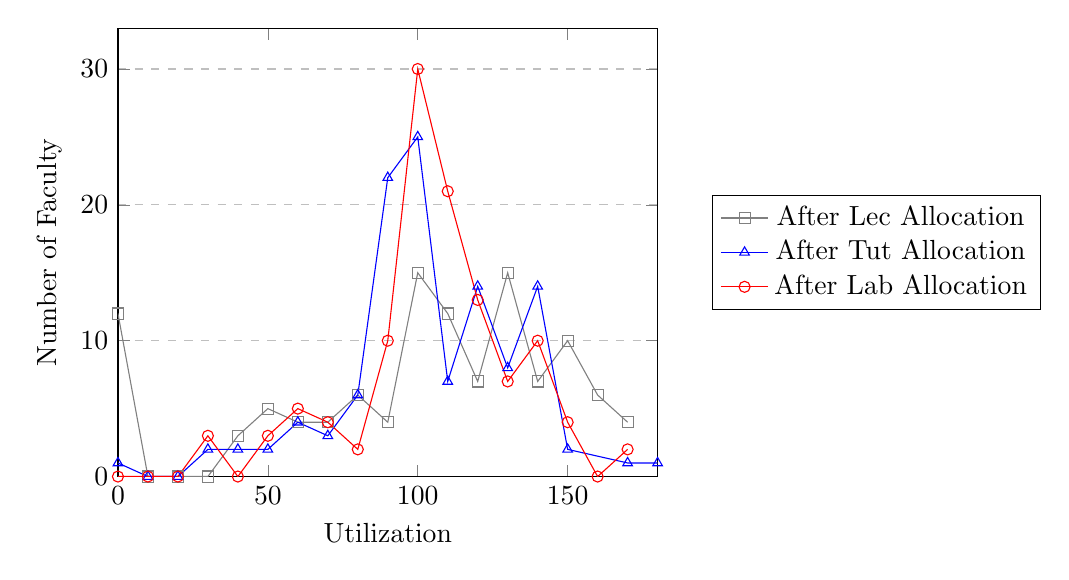
\begin{tikzpicture}
    \begin{axis}[
        xlabel={Utilization},
        ylabel={Number of Faculty},
        xmin=0, xmax=180,
        ymin=0,
        ymajorgrids=true,
        grid style=dashed,
        legend style={at={(1.1,0.5)},
            anchor=west,legend columns=1},
      ]
      \addplot[color=gray, mark=square]
      coordinates {
          (0, 12) (10, 0) (20, 0) (30, 0) (40, 3) (50, 5) (60, 4) (70, 4) (80, 6) (90, 4) (100, 15) (110, 12) (120, 7) (130, 15) (140, 7) (150, 10) (160, 6) (170, 4)
        };
      \addlegendentry{After Lec Allocation}
      \addplot[color=blue, mark=triangle]
      coordinates {
          (0,1) (10,0) (20,0) (30,2) (40,2) (50,2) (60,4) (70,3) (80,6) (90,22) (100,25) (110,7) (120,14) (130,8) (140,14) (150,2) (170,1) (180,1)
        };
      \addlegendentry{After Tut Allocation}
      \addplot[color=red, mark=o]
      coordinates {
          (0, 0) (10, 0) (20, 0) (30, 3) (40, 0) (50, 3) (60, 5) (70, 4) (80, 2) (90, 10) (100, 30) (110, 21) (120, 13) (130, 7) (140, 10) (150, 4) (160, 0) (170, 2)
        };
      \addlegendentry{After Lab Allocation}
    \end{axis}
  \end{tikzpicture}
  \caption{Faculty Utilization for Tutorial Allocation}
  \label{fig:tut_faculty_utilization}
\end{figure}

\autoref{fig:tut_faculty_utilization} shows the utilization of faculty for the tutorial allocation process. The utilization of faculty is defined as the number of hours allocated to the faculty divided by the total workload limit of the faculty. This also means that the utilization of faculty is inclusive of the lecture allocation process, since the lecture allocation process is run before the tutorial allocation process.

One consistent pattern that can be seen in the utilization of faculty is that optimal utilization of faculty, i.e. 100\% utilization, is achieved for more faculty as the tutorial and lab allocation processes are completed, while over-utilized and under-utilized faculty remain nearly constant. This is because many more faculty are available to teach tutorials and labs than lectures, as previously discussed, the broader availability resulting from the lower expertise required to teach tutorials and labs. It can be seen that the number of faculty with 0\% utilization decreases from 12 to 0, which confirms the above finding.

Relatively few faculty are over-utilized, with only 23 faculty having a utilization of more than 120\%. This is because overutilization of faculty in lecture allocation was overutilization of lecture workload limits. But since the workload limits of the faculty are increased to include tutorials and labs, the originally over-utilized faculty are no longer over-utilized.

\subsubsection{Impact of Consistency Bias}

\begin{figure}[H]
  \centering

  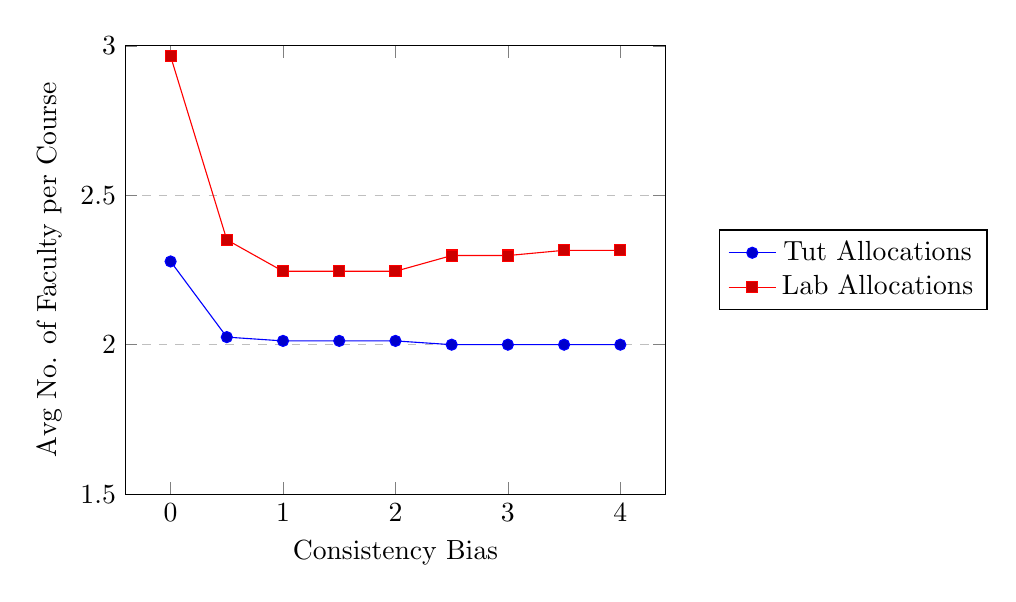
\begin{tikzpicture}
    \begin{axis}[
        xlabel={Consistency Bias},
        ylabel={Avg No. of Faculty per Course},
        ymin=1.5, ymax=3,
        ymajorgrids=true,
        grid style=dashed,
        legend style={at={(1.1,0.5)},
            anchor=west,legend columns=1},
      ]
      \addplot coordinates{
          (0, 2.278481012658228)
          (0.5, 2.0253164556962027)
          (1, 2.0126582278481013)
          (1.5, 2.0126582278481013)
          (2, 2.0126582278481013)
          (2.5, 2.0)
          (3, 2.0)
          (3.5, 2.0)
          (4, 2.0)
        };
      \addlegendentry{Tut Allocations}
      \addplot coordinates{
          (0, 2.9649122807017543)
          (0.5, 2.3508771929824563)
          (1, 2.245614035087719)
          (1.5, 2.245614035087719)
          (2, 2.245614035087719)
          (2.5, 2.2982456140350878)
          (3, 2.2982456140350878)
          (3.5, 2.3157894736842106)
          (4, 2.3157894736842106)
        };
      \addlegendentry{Lab Allocations}
    \end{axis}
  \end{tikzpicture}
  \caption{Impact of Consistency Bias on Faculty per Course}
  \label{fig:tut_consistency_bias}
\end{figure}

TODO: Show the impact of the Yearwise Bias.

TODO: Show the impact of workload limits.

TODO: Show the impact of batching.

TODO: Show the impact of pre-allocation, workload limit relaxation.


\section{Dynamically Adjusting Workload Limits for Feasibility}

% Talks about how the workload limits are dynamically adjusted to ensure that the allocation is feasible. This is done by adjusting the workload limits and the constraint on the total number of teaching activities that can be allocated to each faculty.

% Talks about how this is done through iterative adjustment, detecting if the workload limit or the max allocation limit is responsible for the infeasibility and adjusting the workload limit or the max allocation limit accordingly.

Although the tutorial and lab allocation process manages to allocate most of the tutorials and labs, there are still some tutorials and labs that remain unallocated due to the workload limits of the faculty or the total number of teaching activities that can be allocated to each faculty. This is because the workload limits of the faculty are set to the workload limits of the institution, which are based on the proportion of lectures, tutorials and labs in the institution. However, allocation of all the tutorials and labs is the primary objective of the tutorial and lab allocation process. Thus, the workload limits of the faculty need to be adjusted to accommodate the tutorials and labs that have not been allocated.

To achieve this, a method of dynamically adjusting the workload limits of the faculty is introduced. This involves identifying the cause of the infeasibility, i.e. whether the workload limit of the faculty is responsible for the infeasibility, or whether the total number of teaching activities that can be allocated to each faculty is responsible for the infeasibility. Then, the workload limit of the faculty or the total number of teaching activities that can be allocated to each faculty is adjusted accordingly, to ensure that the allocation is feasible.

This is done by iteratively adjusting the workload limits of the faculty, and then checking if the allocation is feasible. If the allocation is feasible, then the process is complete.

\section{Comprehensive approach to Tutorial and Lab Allocation}

% Describes the entire process of tutorial and lab allocation, along with the figure of the steps involved.

\section{Overview of Course Allocation Process}


\section{Summary}
